\documentclass[a4paper,12pt,twoside]{book}
\usepackage[T1]{fontenc}
\usepackage{inputenc}
\usepackage{fontspec}
\usepackage{lmodern}
\usepackage[english,french]{babel}
\usepackage{xspace} % pour la gestion des espaces après les commandes
\usepackage{minted} % colored source code
\usepackage{csquotes}

% Mise en page École des chartes
\usepackage[margin=2.5cm]{geometry} % marges
\usepackage{setspace}
\onehalfspacing % interligne de 1.5
\setlength\parindent{1cm}

\usepackage{tocbibind}
\usepackage[backend=biber, sorting=nyt, style=enc, minbibnames=10, maxbibnames=10]{biblatex}
\addbibresource{bibliographie/biblio_astro.bib}
\nocite{*}
\defbibnote{intro}{Cette bibliographie présente toutes les ressources utilisées, de tout type, citées ou non, par simple ordre alphabétique.}

\usepackage[pdfusetitle, pdfsubject={Mémoire TNAH — Titre}, pdfkeywords={mot1, mot2, mot3}]{hyperref}

\usepackage{graphicx}
\usepackage{subcaption}

\author{Prénom Nom – M2 TNAH — ENC}
\title{Titre mémoire}

% ACRONYMS
\usepackage[automake, acronym, toc]{glossaries}
\makeglossaries
\setacronymstyle{short-long}
\newacronym{fair}{\textsc{fair}}{\emph{Findable Accessible Interoperable Reusable}}
\newacronym{api}{\textsc{api}}{\emph{Application Programming Interface}}

% COMMANDS
\newcommand{\enc}{École nationale des chartes\xspace}
\newcommand{\fair}{\gls{fair}\xspace}
\newcommand{\api}{\gls{api}\xspace}
\newcommand{\XIV}{\textsc{xiv}\ieme{}\xspace}
% Pour retirer le titre courant d'une page vide avant un chapitre
\newcommand{\clearemptydoublepage}{\newpage{\pagestyle{empty}\cleardoublepage}}
% Pour des sections non numérotées dans la table des matière
\newcommand\chapterNo[1]{
	\chapter*{#1}
	\markright{\MakeUppercase{#1}}
}


\begin{document}
	
	\onehalfspacing 
	
	\frontmatter
	
	\begin{titlepage}
	\begin{center}
		
		\bigskip
		
		\begin{large}
			ÉCOLE NATIONALE DES CHARTES
		\end{large}
		\begin{center}\rule{2cm}{0.02cm}\end{center}
		
		\bigskip
		\bigskip
		\bigskip
		\begin{Large}
			\textbf{Lucie Ledieu}\\
		\end{Large}
		\begin{normalsize} \textit{licencié/maître ès ***}\\
		\end{normalsize}
		
		\bigskip
		\bigskip
		\bigskip
		
		\begin{Huge}
			\textbf{Explorer les réseaux de transmission de données historiques}\\
		\end{Huge}
		\bigskip
		\bigskip
		\begin{LARGE}
			\textbf{Elaboration de visualisations pour l'application AIKON}\\
		\end{LARGE}
		
		\bigskip
		\bigskip
		\bigskip
		\begin{large}
		\end{large}
		\vfill
		
		\begin{large}
			Mémoire 
			pour le diplôme de master \\
			\og Technologies numériques appliquées à l'histoire~\fg\\
			\bigskip
			2025
		\end{large}
		
	\end{center}
\end{titlepage}
	
	\thispagestyle{empty}	
	\cleardoublepage
	
	\chapterNo{Résumé}
\addcontentsline{toc}{chapter}{Résumé}
\medskip	

Résumé\\

\textbf{Mots-clés~:} mot1~; mot2~; mot3~.\\

\textbf{Informations bibliographiques~:} Prénom Nom, \textit{Titre du mémoire}, mémoire de master \og Technologies numériques appliquées à l'histoire~\fg, dir. Prénom Nom, École nationale des chartes, 20**.

\clearemptydoublepage
	
	\chapterNo{Remerciements}
	\addcontentsline{toc}{chapter}{Remerciements}
	
	\chapterNo{Introduction}
	\addcontentsline{toc}{chapter}{Introduction}
	
	La mission principale de ce stage était de concevoir des preuves de concept pour des visualisations à partir des données des projets EIDA et VHS. Ces dernières ont pour but de tester la faisabilité et la pertinence de visualisations à intégrer au sein de l’application de traitement semi-automatique de données AIKON. Avant de les développer, j’ai rédigé un cahier des charges et un benchmark des solutions techniques envisageables. Ces livrables techniques m’ont permis de définir des objectifs clairs ainsi que les limites de mon projet. Afin de bien comprendre le fonctionnement de l’application AIKON et l’expérience utilisateur qu’elle procure, j’ai rédigé une documentation pour les différentes fonctionnalités de l’interface utilisateur. Pour clore ce stage, un Digital Humanities Seminar a été organisé pour partager aux chercheurs mes recherches, les différentes étapes de réalisation des visualisations et les résultats obtenus. Plus largement, ce travail m’a amené à réaliser une réflexion approfondie autour du concept de visualisation des données en sciences humaines et sociales que je vais exposer dans ce mémoire. 
	
	
	\thispagestyle{empty}
	\cleardoublepage
	
	\mainmatter
	
	\part{Enjeux scientifiques et techniques de l'analyse automatisée des transmissions iconographiques}
	\chapter{Les diagrammes astronomiques comme objets d'étude des circulations visuelles}
	\section{Les sources astronomiques : un corpus idéal pour l'étude des transmissions}
	\include{templates/section}

	
	Claude Ptolémée est un astronome appartenant à l'école d'Alexandrie dont nous ne connaissons presque rien de sa vie personnelle. Il serait né vers 90 de notre ère et mort vers 168. Il est considéré comme le dernier grand astronome grec de son époque à un moment où l'astronomie a peu évolué depuis Hipparque qui a vécu entre 147 et 127 avant notre ère. Il doit sa renommée dans le monde scientifique grec de son époque grâce au modèle ptolémaïque dont il est le théoricien. Il s'agit d'un modèle géocentrique de l'univers qui place la Terre au centre du monde. Il expose cette théorie dans son ouvrage le plus connu, la \textit{Grande Syntaxe mathématique}, désignée le plus souvent sous le nom d'\textit{Almageste}\footcite{verdetLaubeLastronomieLaurore1990}. Cette oeuvre contient un catalogue des étoiles, un traité complet de trigonométrie plane et sphérique, une liste des instruments essentiels à avoir dans un observatoire et une partie consacrée aux mouvements des astres où il expose sa thèse selon laquelle l'univers est organisé en un modèle géocentrique. En effet, il défend l'idée que la Terre est au centre de l'univers et que les différents astres, c'est-à-dire le Soleil, la Lune et les planètes, gravitent autour d'elle selon des cercles dits épicycles et déférents\footcite{costabelCLAUDEPTOLEMEE90}.
	
	Dans le cadre de notre étude, nous allons analyser la diffusion de ces diagrammes de tradition ptolémaïque présents dans l'\textit{Almageste} dans le temps et dans l'espace. Cette transmission se manifeste déjà à travers l'étymologie du titre l'\textit{Almageste}. En effet, à l'origine appelé \textit{H' math'matik' syntaxis} signifiant « la Grande Syntaxe mathématique », il est transformé en un terme hybride entre l'arabe et le grec signifiant "le plus grand" avant d'être latinisé en "Almagestum"\footcite{raymondjonesPtolemyAccomplishmentsBiography2025}. L'évolution de son titre montre la diffusion de l'oeuvre dans le monde grec et arabe puis plus tard dans l'Occident latin. Nous devons la diffusion de cette oeuvre durant toute la fin de l'Antiquité et la période médiévale à de nombreux traducteurs et commentateurs. Après sa mort deux grands astronomes grecs ont commenté son oeuvre. Théon d'Alexandrie qui aurait vécu autour de 364 de notre ère est l'un des commentateurs de Ptolémée les plus prolifiques. Malheureusement son commentaire de l'Almageste n'a pas entièrement survécu aux différentes époques et certaines parties sont manquantes. Par exemple, le livre III a presque totalement disparu de la tradition manuscrite de l'oeuvre et il est souvent remplacé par une réécriture de Nicolas Cabasilas datant du XIVe siècle. En 1953, le Chanoine Rome retrouve une édition conservée dans un unique manuscrit le \textit{Laurentianus gr. 28/18}. Cependant, il ne reste que des fragments du livre V et le livre XI a entièrement disparu\footcite{tihonLivreRetrouveCommentaire1987}* Le livre V retrouvé du \textit{Commentaire à l'Almageste} de Théon d'Alexandrie. A peu près à la même époque, vers 340 de notre ère, le mathématicien Pappus d'Alexandrie rédige un commentaire de l'\textit{Almageste} dans le livre IV de ses \textit{Collections mathématiques}, ouvrage dans lequel il expose de manière complète et systématique toutes les connaissances de son époque en apportant des explications ou des approfondissements\footcite{meyerPAPPUS1999}. Plusieurs siècles plus tard, Gérard de Crémone importe l'oeuvre de Ptolémée dans l'Occident chrétien. Il réalise une traduction latine de l'\textit{Almageste} en 1213 à Paris avec des annotations\footcite{ptolemaeusPtolomeusAlmagestumTransl1213}* Gallica. Dans l'une des initiales historiées du manuscrit, nous retrouvons une illustration en hommage  à Ptolémée le représentant sous la forme d'un roi trônant en majesté\footcite{TraductionLatineLAlmageste}* Essentiel BNF. Dans le monde arabo-islamique médiéval, le savant persan Mohammad Nasir al-Din al-Tūs rédige un \textit{Tahrir al-Majiṣtī}, ce qui signifie \textit{Commentaire sur l'Almageste}\footcite{universalisMOHAMMADNASIRALDIN2008}* Encyclopedia Universalis. 
	 Averroès rédige également un \textit{Abrégé de l'Almageste} en 1159-1162. La particularité de cette oeuvre vient du fait qu'elle ait été écrite dans un contexte de contestation de l'astronomie ptoléméenne en Andalousie au XIIe siècle. En effet, des savants comme Maïmonide, Ibn Bajja ou Ibn Tufayl pensaient qu'il était nécessaire de réformer les idées de Ptolémée pour qu'elles concordent parfaitement avec la vision aristotélicienne du monde. Averroès faisait parti de ce mouvement mais lorsqu'il rédige l'\textit{Abrégé de l'Almageste}, il n'a pas la volonté de corriger l'oeuvre. En effet, il préfère attendre l'apparition d'une astronomie ptolémaïque entièrement réformée et en attendant il se résigne à suivre les idées communément admises au sujet de l'oeuvre de Ptolémée. Même s'il n'est pas dans une optique de correction des pensées de Ptolémée, Averroès n'est pas astronome et il se peut qu'il fasse quelques erreurs. Néanmoins, ces dernières restent sans gravité car il possède tout de même une bonne connaissance des mathématiques. *Averroès : abrégé d'astronomie dans la version hébraïque (position de thèse) Nous ne possédons qu'une version traduite en hébreu par Jacob Anatoli dans le cadre du mécénat de l'empereur Frédéric II au XIIIe siècle. Il n'existe plus aucun témoin de la version arabe et il semblerait que cette dernière n'est jamais été traduite en latin\footcite{layAverroesHebraicusInedit2005}* Un Averroes hebraicus inédit.
	
	Ces différentes traductions et commentaires montrent l'étendue de la diffusion de l'oeuvre à travers les siècles dans le monde entier. La vision géocentrique de l'univers de Ptolémée ne sera remise en question qu'au XVIe siècle suite aux travaux de Copernic. Dans son \textit{De Revolutionibus orbium caelestium}, il défend la thèse de l'héliocentrisme dans laquelle le Soleil se trouve au centre du monde\footcite{verdetHELIOCENTRISME2008}* Encyclopedia Universalis heliocentrisme.
	
	
	
	
	\section{L'iconographie comme témoin des diffusions intellectuelles}
	\include{templates/section}

	
	Nous pouvons regrouper les diagrammes en différentes familles. Néanmoins, les frontières de ces dernières ne sont pas totalement étanches. Il se peut que certains diagrammes aient des caractéristiques de plusieurs familles à la fois. Les diagrammes mathématiques servent à représenter des concepts géométriques ou arithmétiques par l'usage spécifique d'idiomes, de lignes, de cercles et d'étiquettes alphabétiques. Ils servent par exemple à calculer la position d'une planète ou d'une étoile. Les diagrammes astrologiques montrent la position des astres à un moment donné pour en tirer des prédictions ou des interprétations sur les activités humaines. Ils sont dessinés à l'aide de lignes, cercles et d'un langage graphique. Les diagrammes d'instrument permettent de comprendre le fonctionnement ou la structure d'un instrument astronomique comme l'astrolabe ou le quadrant afin de réaliser une observation ou un calcul. Ils sont représentés à l'aide de graduations, de nombres, de lignes et de cercles plus métriques. Pour finir, le diagramme cosmologique montre l'organisation de l'univers dans son ensemble par le biais de l'utilisation d'un langage de couleur et de texture. = EIDA conférence 2025
	
	
	
	Dès lors, nous pouvons nous poser la question suivante : Ces éléments iconographiques doivent-il être réduits à une fonction démonstrative et explicative ou peuvent-ils être exploités pour retracer la diffusion d'une oeuvre au même titre que le texte lui-même ?
	
	En 2014, Dominique Raynaud publie un article nommé \textit{"Building the stemma codicum from geometric diagrams. A treatise on optics by Ibn al-Haytham as a test case"} dans lequel il expose une idée novatrice : il veut établir un stemma codicum d'une tradition écrite uniquement à partir de diagrammes\footcite{raynaudBuildingStemmaCodicum2014}.
	
	Un stemma codicum est la représentation de toutes les étapes de la transmission d'une oeuvre sous la forme d'un arbre inversé en établissant des relations entre les différents manuscrits. Le but de l'éditeur est alors de reconstituer le texte le plus proche du manuscrit original perdu que l'on nomme "archétype". Il s'agit de l'ancêtre commun le plus récent d'une oeuvre. En effet, lorsqu'un texte est copié à plusieurs reprises, il constitue une "tradition littéraire" dont les exemplaires sont nommés "témoins" dans le domaine de la philologie. Pour tenter de reconstituer le "stemma codicum" il est donc nécessaire de relever les différentes variantes provenant des divers manuscrits\footcite{pouliquenUsingLatticesReconstructing} * using lattices.
	
	Pour établir un stemma codicum à partir de diagrammes, Dominique Raynaud emprunte à la biologie le principe de cladistique. Il s'agit "d'une méthode de classification biologique qui exprime la phylogénie, c'est à dire les relations de parenté existant entre les êtres vivants". Cette méthode "repose sur le partage de caractères hérités d'une ascendance commune", c'est-à-dire d'un "ancêtre commun"\footcite{tassyCLADISTIQUE2012}. *Encyclopedia Universalis
	
	Il explique que pour étudier les différents témoins d'une oeuvre et les traditions qui l'entourent, il faut se baser sur les erreurs afin de réaliser un arbre généalogique. Nous pouvons affirmer que par cette démarche, il choisit d'utiliser la méthode Lachmann. Il s'agit d'une méthode philologique élaborée au XIXe siècle par le philologue allemand Karl Lachmann dite de l'erreur commune. Ce dernier défendait la thèse suivante : Si un des témoins du texte présente une erreur, alors il y a de fortes chances que cette erreur soit aussi présente dans son descendant\footcite{pouliquenUsingLatticesReconstructing} *Using lattices .
	
	Dans son article, Dominique Raynaud teste sa méthode sur un traité d'optique d'Ibn al-Haytham. En suivant cette méthode, il est arrivé à constituer le premier stemma de diagrammes jamais publié. Il a été réalisé à partir des cinq témoins contenant l'oeuvre : 
	
	
	\begin{figure}[h]
		\centering
		\begin{subfigure}{0.48\linewidth}
			\centering
			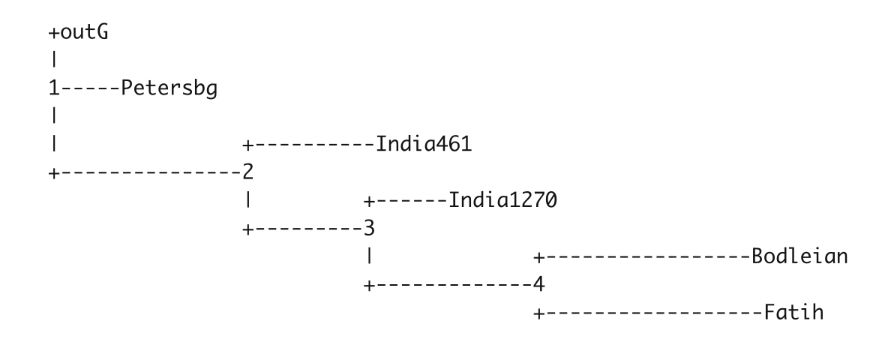
\includegraphics[width=\linewidth]{images/diagram_stemma.png}
		\end{subfigure}
		\hfill
		\begin{subfigure}{0.48\linewidth}
			\centering
			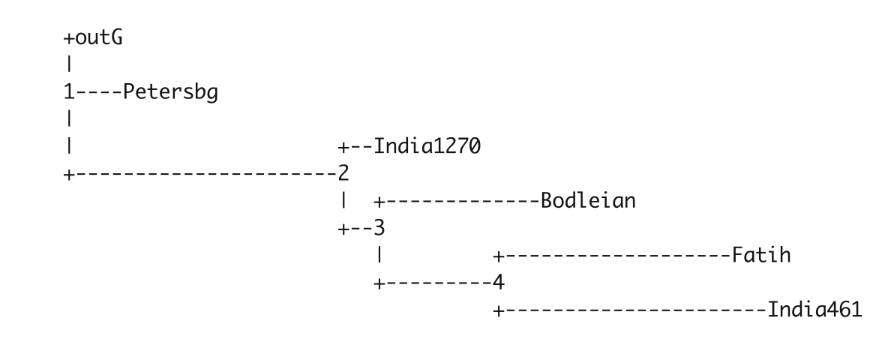
\includegraphics[width=\linewidth]{images/text_stemma.png}
		\end{subfigure}
		\caption{Stemma pour les diagrammes - Stemma pour le texte \footcite{raynaudBuildingStemmaCodicum2014}}
		\label{fig:stemma}
	\end{figure}

	
	En y regardant plus en détail, nous pouvons voir qu'il y a une forte similitude entre le stemma textuel et le stemma des diagrammes. Il en vient à la conclusion suivante : Quand les diagrammes sont intégrés au texte, il est envisageable de ne faire qu'un seul arbre pour les deux. Néanmoins, si les diagrammes ont été copiés a posteriori du texte ou qu'ils ont été corrigés par la suite, mieux vaut réaliser deux stemmata distincts et étudier leur transmissions séparément. Le fait qu'ils aient été copiés par des personnes différentes à des moments différents impacte fortement leur étude. Selon lui, il est même plus avantageux de réaliser le stemma codicum d'une tradition mathématique. La densité d'erreur serait sept à huit fois plus élevée dans un diagramme géométrique que dans un texte occupant la même superficie. Dans la mesure où sa méthode repose sur le relevé d'erreurs, il est plus judicieux de réaliser un stemma avec des diagrammes\footcite{raynaudBuildingStemmaCodicum2014}.* Dominique Raynaud.
	
	
	\section{Limites des approches philologiques traditionnelles}
	\include{templates/section}
	
	Le travail philologique peut s'avérer plus compliqué lorsqu'un même concept ou démonstration peuvent être représentés de plusieurs façons.
		
	En effet, les conventions et les choix graphiques pour la représentation des diagrammes a évolué au fil du temps et des aires géographiques. Michela Malpangotto a étudié ce phénomène en s'appuyant sur l'exemple de l'oeuvre de Théodose les \textit{Sphériques} écrit au Ier siècle avant notre ère. Il s'agit d'un texte fondamental dans l'étude de la géométrie sphérique est structuré en 59 propositions et divisé en trois livres. Il fait partie de ce que l'on nomme la "Petite astronomie", un recueil d'ouvrages compilés par les Grecs afin de faciliter la compréhension de l'Almageste de Ptolémée. Il a été étudié et transmis pendant près de dix siècles. La géométrie sphérique est définit de la manière suivante : \og La géométrie sphérique étudie la sphère comme un objet solide mais surtout comme contexte spatial des éléments qui interagissent sur elle dans un agencement tridimensionnel complexe. \fg Il est alors nécessaire de mettre au même niveau, le plan du diagramme et l'agencement spatial des objets autour de la sphère. Cette dernière est un objet solide mais elle est surtout un contexte spatial pour les arcs, les segments de droites et des cercles qui y sont déterminés par l'intersection de différents plans inclinés dans l'agencement spatial tridimensionnel. 
	
	Dans la version grecque originale, les deux parties de l'oeuvre sont séparées par le choix de l'iconographie des diagrammes. Dans la première partie, nous retrouvons des diagrammes dans lesquelles la sphère n'est pas représentée. Il y a seulement des cercles produits par l'intersection du plan incliné de différentes manières qui sont représentés de manière juxtaposés dans le plan du diagrammes. Les arcs ainsi que les segments linaires sont aplatis et les objets placés de l'autre côté de la sphères sont retournés dans le plan de la figure. La conséquence majeure de cette manière de représentation est la dépendance des diagrammes vis-à-vis du texte. Il est nécessaire de lire les explications pour comprendre le diagramme. Dans la seconde partie de l'oeuvre, les diagrammes sont construits en utilisant la perspective. Nous pouvons donc observer les éléments géométriques interagir entre eux à l'intérieur de cette dernière.  
	
	En Italie, Platon de Tivoli a réalisé trois éditions de cette oeuvre au XVIe siècle en s'appuyant sur une version arabo-latine médiévale. Il choisit de représenter les diagrammes de manière schématique et plane comme dans la première partie de la version grecque originale de l'oeuvre. 
	
	L'édition de Francesco Maurolico marque un tournant dans la transmission des Sphériques. En effet, ce dernier fait le choix de travailler sur la surface de la Sphère qui, mise en avant, devient le contexte réel dans lequel les éléments géométriques interagissent. Christophe Clavius, un mathématicien allemand adopte cette iconographie dans son édition de 1586 qui sert de base à la tradition moderne des \textit{Sphériques}\footcite{malpangottoGraphicalChoicesGeometrical2010}. * insérer source 
	
	\begin{figure}[h]
		\centering
		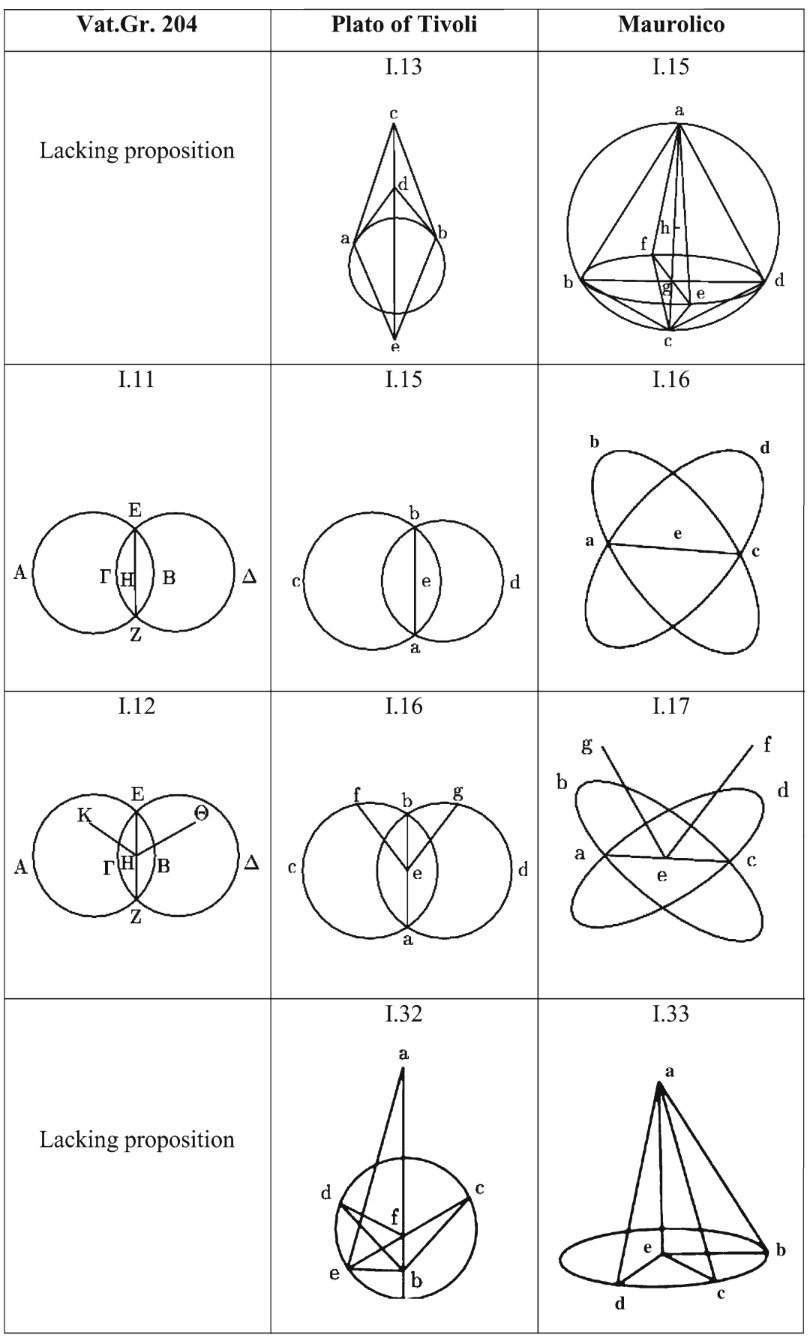
\includegraphics[width=0.9\linewidth]{images/conventions_diagrammes.png}
		\caption{Différentes conventions de représentation de diagrammes de l'étude de Michela Malpangotto\footcite{malpangottoGraphicalChoicesGeometrical2010}}
		\label{fig:conventions}
	\end{figure}
	
	
	
	
	\clearemptydoublepage
	
	\chapter{AIKON et l'automatisation des traitements}
	\section{Le choix de la vision artificielle pour ces objets d'étude : la plateforme AIKON}
	\include{templates/section}
	
	\section{Extraction de regions / Calcul de similarités}
	\include{templates/section}
	
	\section{De l'annotation manuelle au traitement de masse : les interfaces existantes}
	\include{templates/section}
	
	\clearemptydoublepage
	
	\chapter{Vers la nécessité d'interfaces d'exploration}
	\section{Masse de données et limites de l'exploration manuelle}
	\include{templates/section}
	
	\section{De la correction d'annotations à l'interprétation scientifique}
	\include{templates/section}
	
	\section{Questions de recherche et besoins d'exploration du corpus}
	\include{templates/section}
	
	\clearemptydoublepage
	
	
	\part{Méthodologie de conception des visualisations exploratoires}
	\chapter{La visualisation en histoire}
	\section{Evolution des représentations visuelles en histoire}
	\include{templates/section}
	
	\section{Visualisations de réseaux et étude des disséminations}
	\include{templates/section}
	
	\section{Enjeux critiques de la médiation numérique des données historiques}
	\include{templates/section}
	
	\clearemptydoublepage
	
	\chapter{Formalisation des besoins et contraintes de conception}
	\section{Analyse des pratiques et questions des chercheurs EIDA}
	\include{templates/section}
	
	\section{Cahier des charges : objectifs scientifiques et contraintes techniques}
	\include{templates/section}
	
	\section{Choix méthodologiques : network graph et alignement des sources (bipartite)}
	\include{templates/section}
	
	\clearemptydoublepage
	
	\chapter{Processus itératif de développement}
	\section{Prototypage et tests de faisabilité technique}
	\include{templates/section}
	
	\section{Mise en oeuvre concrète : choix techniques et difficultés rencontrées}
	\include{templates/section}
	
	\section{Intégration des retours utilisateurs et ajustements}
	\include{templates/section}
	
	\clearemptydoublepage
	
	\part{Evaluation critique et perspectives d'intégration}
	\chapter{Analyse des visualisations produites}
	\section{Visualisation bipartite : révéler les réorganisations du contenu intellectuel}
	\include{templates/section}
	
	\section{Network graph : explorer les chaînes de transmissions}
	\include{templates/section}
	
	\section{Adéquation aux objectifs d'exploration scientifique}
	\include{templates/section}
	
	\clearemptydoublepage
	
	\chapter{Validation et limites méthodologiques}
	\section{Critères d'évaluation de l'efficacité exploratoire}
	\include{templates/section}
	
	\section{Retour d'expérience par les chercheurs}
	\include{templates/section}
	
	\section{Limites liées aux données et biais d'interprétation}
	\include{templates/section}
	
	\clearemptydoublepage
	
	\chapter{Perspectives d'évolution et généralisation}
	\section{Intégration dynamique à la plateforme AIKON}
	\include{templates/section}
	
	\section{Transférabilité vers d'autres corpus et projets}
	\include{templates/section}
	
	\section{Implications pour l'évolution des pratiques en humanités numériques}
	\include{templates/section}
	
	\clearemptydoublepage
	
	\chapterNo{Conclusion}
	\addcontentsline{toc}{chapter}{Conclusion}
	
	\appendix
	\part*{Annexes}	
	\addcontentsline{toc}{part}{Annexes}
	
	\clearemptydoublepage
	
	\backmatter
	\printacronyms[title=Liste des acronymes,toctitle=Acronymes]
	\printglossary 
	\printbibliography
	\tableofcontents
	
\end{document}